% !TeX root = ../../Thesis.tex
\chapter{Effects of laser bandwidth on inflationary stimulated Raman scattering}
\label{chp:broadbandSRS}

\section{Motivation and literature review}

\subsection{Original idea that bropadband might control LPI}
Early results in the 1970s suggested that finite-bandwidth laser drivers could change the behaviour of parametric instabilities. These studies considered a variety of parametric instabilities, including: the parametric decay instability \citep{Thomson1974}; stimulated Brillouin scattering \citep{Kruer1973};  


We expect broadband to affect absolute SRS at $0.25n_{\text{cr}}$ in this way. \citet{Follet_2019} use LPSE to treshodl for absolute SRS in ICF, and find that they can be increased for a continuous broadband spectrum with random spectral phases, as correlation time of the pump increase

\subsection{Different models of broadband}
\subsection{Smoothing by spectral dispersion}

SSD,ISI,SRRS,whater Gudzar did

\subsection{Stimulated rotational Raman scattering}
Here \citep{Eimerl1993} and here \citep{Weaver2017} (theoretical model for SRRS)

\subsubsection{Decoupled broadband lasers}
In \cite{zhao_suppression_2019} they consider the suppression of parametric
instabilities in a homogeneous plasma by decoupled broadband lasers
(\acrshort{DBL}). A
decoupled broadband laser is defined in Ref \cite{zhao_effective_2017} as

\begin{equation}\label{eqn:DBL}
  a_{\mathrm{DBL}} = \sum_{i=1}^{N} a_i \mathrm{cos}(\omega_it + \phi_i),
\end{equation}
where $a_i,\omega_i,\phi_i$ are the amplitude, carrier frequency, and phase of
each of the $N$ beamlets. The central frequency and wavelength of the laser is
$(\omega_0,k_0)$ and the total frequency spectrum bandwidth is
$\Delta\omega_0$.
Considering the frequency difference between any two beamlets, they find that
there is a critical frequency difference below which the SRS instability regions
for the beamlets overlap to form a single instability region. In this case, the
two beamlets can be coupled with one EPW, leading to a higher growth rate for
SRS. An important result of their one-dimensional PIC simulations is that iSRS
instability can grow to a high level if the beamlets satifsy this coupling
condition, even if the total bandwidth is very large.

\subsubsection{Strongly kinetic regime}
In Ref \cite{zhou_kinetic_2018} Zhou \textit{et al.} consider the case of SRS
driven by a broadband laser for a homogeneous plasma, with NIF-relevant plasma
density and temperature such that $\kld > 0.3$. The result most relevant to our
work is that the bandwidth can interact with the nonlinear frequency shift associated
with electron trapping in the SRS EPW to \emph{enhance} SRS rather than suppress it.


\subsection{Decoupled broadband lasers}
Zhao \textit{et al.} \cite{zhao_effective_2017} consider the case of an
inhomgeneous plasma density profile relevant to indirect-drive ICF. The results
are similar to those described in the homogeneous case, and they find a
condition for the complete suppression of SRS. The follow-up paper
\cite{zhao_suppression_2019} finds that SRS can be well controlled for a laser
beam structure of multiple frequency components and total bandwidth of a few
percent. The parameters considered in this study are
$\lambda_0=0.33\si{\micro\metre}$,
$T_e=2\si{\kilo\electronvolt}$, $n_e = [0.08,0.12]n_c$, giving $\kld \sim
[0.26,0.35]$, well within the kinetic regime for SRS.

They derive a gain exponent for standard convective SRS driven by two
beamlets of different frequencies, and find that two beamlets are independent
when
\begin{equation}\label{DLB_threshold_inhomo}
\delta \omega_{0} \geq \frac{\pi n_{0} c\left(\omega_{0}^{2}-\omega_{p
e}^{2}\right)^{3 / 2}}{8 L \omega_{0} \omega_{L}^{2} \nu_{p}^{2}}.
\end{equation}
Importantly, this condition is independent of the amplitude of the incident
laser. In theory, this condition would allow us to construct a DBL to suppress
SRS in a large-scale inhomogeneous plasma, however, secondary amplification of
back-scattered light by one of the beamlets is a possibility. We must therefore
consider another threshold for this secondary amplification: $\delta\omega_0 >
\omega_{L1}-\omega_{L2}$ where $[\omega_{L1},\omega_{L2}]$ is the range of EPW
frequencies excited by SRS in the plasma (not including nonlinear frequency
shift).



\subsection{Continuous bandwidth}
We can implement a continuous-bandwidth frequency-modulated laser in EPOCH using the standard EPOCH laser-driver,

\begin{equation}
 	 E(x,t) = E_0\text{sin}\left(\omega_0 t - \phi(x,t)\right),
\end{equation} with $\phi(x,t)$ is given by

\begin{equation}
	\phi(x,t) = \frac{1}{2}\frac{\Delta\omega}{\omega_m}\text{sin}	 	 \left(\omega_mt - \frac{\omega_m}{c}x\right).
\end{equation}

\section{Evidence of effect on SRS}
The intro of this basically tells me everything I need to know \citep{Follett2021}

In the case of absolute SRS in inhomogeneous plasma, the absolute instability threshold can be increased by using bandwidth.

\citet{Guzdar1991} says that the convective gain of SRSis not senstivie to bandwidth. However there are a range of additional effect which can determine the gain of convective SRS which can be mitigated by broadband. These include: increasing the threshold for inflationary SRS driven by a laser with SSD-type bandwidth; mitigating speckle self-focussing.

Studies have also been performed using the code LPSE which show that, at ignition scales, absolute multi-beam backward SRS can be mitigated with bandwith $\sim 1.6\%$ \citep{Follett2021}.

\section{1D simulations and threshold}
We begand this study by replicating the results of WEN PREPRINT which claims that 

\begin{table}[]
\begin{tabular}{|l|l|l|}
\hline
\textbf{gain medium} & \textbf{\begin{tabular}[c]{@{}l@{}}wavelength\\       (nm)\end{tabular}} & \textbf{\begin{tabular}[c]{@{}l@{}}bandwidth\\         (THz)\end{tabular}} \\ \hline
Nd : glass           & 351                                                                      & 1                                                                                \\ \hline
KrF                  & 284                                                                      & 3                                                                                \\ \hline
ArF                  & 193                                                                      & 10                                                                               \\ \hline
\end{tabular}
\end{table}


\begin{figure}[ht]
   \centering
    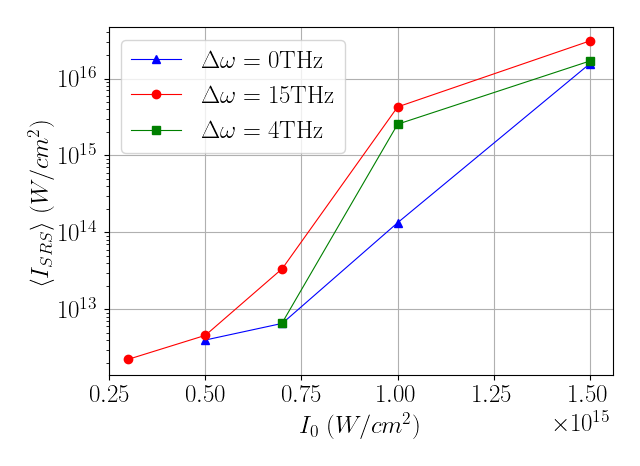
\includegraphics[width=0.75\columnwidth]{Chapters/C5_broadband/bandwidth_no_dependence_Wen.png}
    \caption{Intensity of light scattered by SRS, averaged over the last three picoseconds of each simulation, for three laser set-ups with fixed maximum normalised chirp ($\Delta\omega \omega_m / \omega_0=5.5\times10^{-6}$) and varied bandwidth. The simulation parameters common to all data-points are: $T_e = 4\si{\kilo eV}; L_n = 400\si{\micro\metre}; n_e(x) = 0.11n_{\text{cr}}\text{exp}(x/L_n);\text{PPC=16,000}. $}
    \label{fig:pumpdepletion}
\end{figure}{}


\section{2D simulations}



%\bibliographystyle{plainnat}
%\bibliography{Chapters/C5_broadband/broadband}
